\chapter{Specifikacija programske potpore}
		
	\section{Funkcionalni zahtjevi}
			
			\textbf{\textit{dio 1. revizije}}\\
			
			\textit{Navesti \textbf{dionike} koji imaju \textbf{interes u ovom sustavu} ili  \textbf{su nositelji odgovornosti}. To su prije svega korisnici, ali i administratori sustava, naručitelji, razvojni tim.}\\
				
			\textit{Navesti \textbf{aktore} koji izravno \textbf{koriste} ili \textbf{komuniciraju sa sustavom}. Oni mogu imati inicijatorsku ulogu, tj. započinju određene procese u sustavu ili samo sudioničku ulogu, tj. obavljaju određeni posao. Za svakog aktora navesti funkcionalne zahtjeve koji se na njega odnose.}\\
			
			
			\noindent \textbf{Dionici:}
			
	\begin{packed_enum}
				\item  Neregistrirani korisnik
				\item  Registrirani korisnik 
					\begin{packed_enum}
						
						\item  klijent
						\item  klub
						\item  trener
						\item administrator
				
					\end{packed_enum}

				\item Razvojni tim
				\item Asistenti
										
			\end{packed_enum}
			
			\noindent \textbf{Aktori i njihovi funkcionalni zahtjevi:}
			
			
			\begin{packed_enum}
				\item  \underbar{ Neregistrirani korisnik (inicijator) može:}
				
				\begin{packed_enum}
					\item pregledati na karti dostupne plesnjake i lokacije klubova
					\item odabrati profile klubova (ime kluba, kontakt telefon, email adresu, kratki opis)  i pregledati tipove plesa (naziv, kratki opis, slika i link na video primjer plesa) koje ti klubovi nude
					\item registrirati se, kreirati novi korisnički račun za klijenta za koji su mu potrebni korisničko ime, lozinka, ime, prezime, spol, datum rođenja, broj mobitela, email adresa i opcionalno opis plesnog iskustva i fotografija
					\item kreirati novi korisnički račun za klub za koji su mu potrebni korisničko ime, lozinka, ime kluba, adresa sjedišta, telefon i email

					
				\end{packed_enum}
			
				\item  \underbar{Klijent (inicijator) može:}
				
				\begin{packed_enum}
					
					\item pregledavati i mijenjati osobne podatke
					\item izbrisati svoj korisnički račun
					\item  pregledati na karti tečajeve slobodne za upis 
					\item odabrati tečaj/grupu i dobiti prikaz relevantnih informacija (vrsta plesa, kalendar s terminima tečaja i lokacijama s dvoranama, ime i prezime te sliku trenera)
					\item poslati prijavu klubu da postane trener koja mora sadržavati motivacijsko pismo i potvrdu u pdf formatu da je osposobljen držati tečaj plesa
					\item pregledati aktivne prijave na tečaj/grupu kluba (informacije o treneru, skupu treninga kroz neko vrijeme, maksimalnom broju sudionika, opis s dodatnim informacijama o težini treninga, uvjetima treniranja i pravilima ponašanja) i prijaviti se

					
				\end{packed_enum}
			
			
				\item  \underbar{Klub (inicijator) može:}
				
				\begin{packed_enum}
					\item organizirati plesnjak uz odgovarajući opis (lokacija, naziv, opis i slika) – lokacija plesnjaka može biti na lokaciji kluba ili izvan nje 
					\item potvrditi klijenta kao trenera
					\item objaviti upise za tečaj/grupu s krajnjim rokom prijave i ograničenjem na dob i spol
					\item odabrati klijente koji se primaju na tečaj/grupu 
					\item naknadno mijenjati popis klijenata
					\item uređivati i brisati tečajeve/grupe
					\item pregledavati i mijenjati osobne podatke
					\item izbrisati svoj korisnički račun 

				\end{packed_enum}
			

			
				\item  \underbar{Trener (inicijator) može:}
				
				\begin{packed_enum}
					
					\item imati podstranicu na kojoj vidi popis tečajeva/grupa koje trenira
					\item vidjeti na kalendaru sve termine tečajeva/grupa koje vodi
					\item vidjeti opće informacije tečaja/grupe za kojeg je zadužen i popis klijenata koji bi trebali biti nazočni na tečaju/grupi

				\end{packed_enum}
			

			
				\item  \underbar{Administrator (inicijator) može:}
				
				\begin{packed_enum}
					
					\item može dodati, mijenjati i brisati plesove
					\item  odobriti prijavu kluba za korištenje aplikacije 
					\item pregledati popis svih klijenata i klubova
					\item uređivati korisničke račune

					
				\end{packed_enum}
			
			
				\item  \underbar{Baza podataka(sudionik) može:}
				
				\begin{packed_enum}
					
					\item pohranjuje sve podatke o korisnicima i njihovim ovlastima
					\item pohranjuje sve podatke o plesnim tečajevima i plesnjacima, njihovim lokacijama i opisima

					
				\end{packed_enum}
			\end{packed_enum}
			
			\eject 
			
			
				
			\subsection{Obrasci uporabe}
				
				\textbf{\textit{dio 1. revizije}}
				
				\subsubsection{Opis obrazaca uporabe}
					\textit{Funkcionalne zahtjeve razraditi u obliku obrazaca uporabe. Svaki obrazac je potrebno razraditi prema donjem predlošku. Ukoliko u nekom koraku može doći do odstupanja, potrebno je to odstupanje opisati i po mogućnosti ponuditi rješenje kojim bi se tijek obrasca vratio na osnovni tijek.}\\
					
					%ovaj dio cu ostaviti za copy-paste template
					\noindent \underbar{\textbf{UC$<$broj obrasca$>$ -$<$ime obrasca$>$}}
					\begin{packed_item}
	
						\item \textbf{Glavni sudionik: }$<$sudionik$>$
						\item  \textbf{Cilj:} $<$cilj$>$
						\item  \textbf{Sudionici:} $<$sudionici$>$
						\item  \textbf{Preduvjet:} $<$preduvjet$>$
						\item  \textbf{Opis osnovnog tijeka:}
						
						\item[] \begin{packed_enum}
	
							\item $<$opis korak jedan$>$
							\item $<$opis korak dva$>$
							\item $<$opis korak tri$>$
							\item $<$opis korak četiri$>$
							\item $<$opis korak pet$>$
						\end{packed_enum}
						
						\item  \textbf{Opis mogućih odstupanja:}
						
						\item[] \begin{packed_item}
	
							\item[2.a] $<$opis mogućeg scenarija odstupanja u koraku 2$>$
							\item[] \begin{packed_enum}
								
								\item $<$opis rješenja mogućeg scenarija korak 1$>$
								\item $<$opis rješenja mogućeg scenarija korak 2$>$
								
							\end{packed_enum}
							\item[2.b] $<$opis mogućeg scenarija odstupanja u koraku 2$>$
							\item[3.a] $<$opis mogućeg scenarija odstupanja  u koraku 3$>$
							
						\end{packed_item}
					\end{packed_item}
					%kraj template-a
					
					\noindent \underbar{\textbf{UC25 -Slanje prijave za trenera}}
					\begin{packed_item}
	
						\item \textbf{Glavni sudionik: }Klijent
						\item  \textbf{Cilj:} Klijent šalje prijavu određenom klubu kako bi postao njihov trener
						\item  \textbf{Sudionici:} Baza podataka, klub
						\item  \textbf{Opis osnovnog tijeka:						
						}
						
						\item[] \begin{packed_enum}
	
							\item Klijent odabire određeni klub
							\item Klijent odabire opciju slanja prijave za trenera
							\item Otvara se prozor sa formom za unos osobnih podataka i datoteka – motivacijsko pismo i potvrda o sposobnosti vođenja tečaja
							\item Klijent unosi podatke i potvrđuje slanje
							\item Podaci se pohranjuju u bazu podataka
							\item Klubu se aplikaciji prikazuje nova prijava
						\end{packed_enum}
						
						\item  \textbf{Opis mogućih odstupanja:}
						
						\item[] \begin{packed_item}
	
							\item[4.a] Podaci u formi imaju krivi format ili nisu ispunjena obavezna polja
							\item[] \begin{packed_enum}
								
								\item Aplikacija obavještava klijenta da unese ispravne i obavezne podatke
																
							\end{packed_enum}
														
						\end{packed_item}
					\end{packed_item}
					
					
					\noindent \underbar{\textbf{UC26 – Potvrda prijave za trenera}}
					\begin{packed_item}
	
						\item \textbf{Glavni sudionik: }Klub
						\item  \textbf{Cilj:} Klijent postaje trener u određenom klubu
						\item  \textbf{Sudionici:} Baza podataka, klijent
						\item  \textbf{Preduvjet:} Klijent poslao prijavu za trenera
						\item  \textbf{Opis osnovnog tijeka:}
						
						\item[] \begin{packed_enum}
	
							\item Klub odabire prijavu od određenog klijenta
							\item Klub potvrđuje prijavu
							\item Klijentu se dodjeljuju ovlasti trenera
							\item Prijava se označava kao obrađena
						\end{packed_enum}
							
						\end{packed_item}
					\end{packed_item}
					
					\noindent \underbar{\textbf{UC27 - Odbijanje prijave za trenera}}
					\begin{packed_item}
	
						\item \textbf{Glavni sudionik: }Klub
						\item  \textbf{Cilj:} Klijentu se odbija poslana prijava za trenera
						\item  \textbf{Sudionici:} Baza podataka, klijent
						\item  \textbf{Preduvjet:} Klijent poslao prijavu za trenera
						\item  \textbf{Opis osnovnog tijeka:}
						
						\item[] \begin{packed_enum}
	
							\item Klub odabire prijavu od određenog klijenta
$>$
							\item Klub odbija određenog klijentaa
							\item Prijava se označava kao obrađena
						\end{packed_enum}
						\end{packed_item}
					\end{packed_item}
					
					\noindent \underbar{\textbf{UC28 – Pregled vođenih tečajeva}}
					\begin{packed_item}
	
						\item \textbf{Glavni sudionik: }Trener
						\item  \textbf{Cilj:} Vidjeti popis tečajeva koje vodi
						\item  \textbf{Sudionici:} Baza podataka
						\item  \textbf{Preduvjet:} Trener vodi tečaj za određeni klub
						\item  \textbf{Opis osnovnog tijeka:}
						
						\item[] \begin{packed_enum}
	
							\item Trener odabire opciju za prikaz svojih tečajeva
							\item Aplikacije prikazuje popis tečajeva koje trener vodi
							\item Trener odabire određeni tečaj
							\item Prikazuje se naziv tečaja sa opisom i nužnim informacijama o tečaju
						\end{packed_enum}
						
						\end{packed_item}
					\end{packed_item}
				
				
					\noindent \underbar{\textbf{UC29 - Pregled kalendara s vođenim terminima}}
					\begin{packed_item}
	
						\item \textbf{Glavni sudionik: }Trener
						\item  \textbf{Cilj:} Vidjeti kalendar s popisom treninga koje vodi određenog dana i sata
						\item  \textbf{Sudionici:} Baza podataka
						\item  \textbf{Opis osnovnog tijeka:}
						
						\item[] \begin{packed_enum}
	
							\item Trener odabire opciju za prikaz svojih vođenih termina
							\item Prikazuje se kalendar s označenim terminima kada vodi tečaj
						\end{packed_enum}
						\end{packed_item}
					\end{packed_item}
					
					\noindent \underbar{\textbf{UC30 - Pregled polaznika }}
					\begin{packed_item}
	
						\item \textbf{Glavni sudionik: }Trener
						\item  \textbf{Cilj:} Vidjeti popis nazočnih sudionika na tečaju
						\item  \textbf{Sudionici:} Baza podataka
						\item  \textbf{Preduvjet:} Trener vodi odabrani tečaj
						\item  \textbf{Opis osnovnog tijeka:}
						
						\item[] \begin{packed_enum}
	
							\item Trener odabire određeni tečaja iz popisa tečajeva
							\item Prikazuje se popis sudionika na tečaju s osnovnim osobnim podacima
						\end{packed_enum}
						
						\end{packed_item}
					\end{packed_item}
					
				\subsubsection{Dijagrami obrazaca uporabe}
					
					\textit{Prikazati odnos aktora i obrazaca uporabe odgovarajućim UML dijagramom. Nije nužno nacrtati sve na jednom dijagramu. Modelirati po razinama apstrakcije i skupovima srodnih funkcionalnosti.}
				\eject		
				
				\begin{figure}[H]
			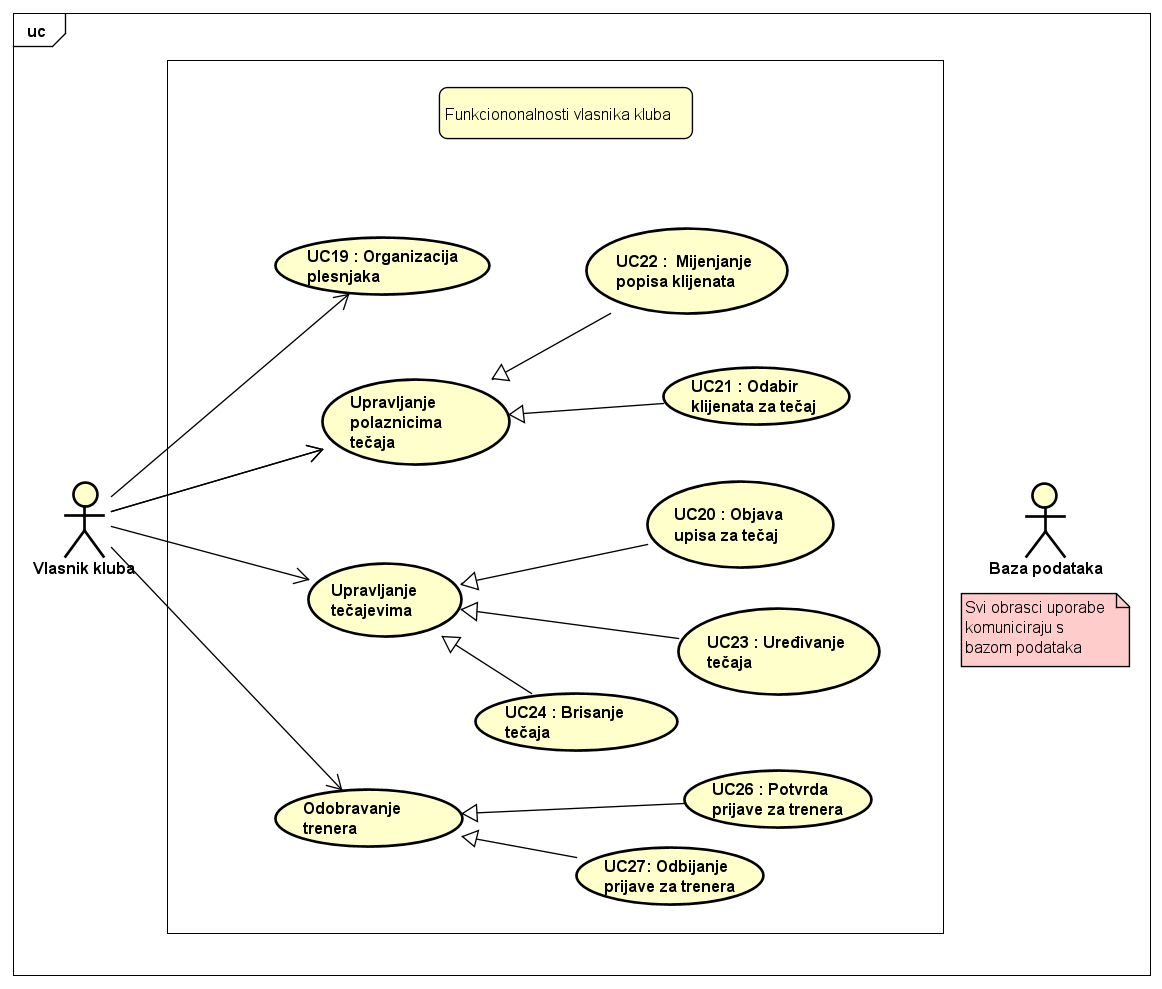
\includegraphics[scale=0.4]{slike/UC_klub.PNG} %veličina u odnosu na širinu linije
			\caption{Dijagram obrasca uporabe, funkcionalnost vlasnika kluba.}
			\label{fig:UC_klub} %label mora biti drugaciji za svaku sliku
		\end{figure}
		
		\begin{figure}[H]
			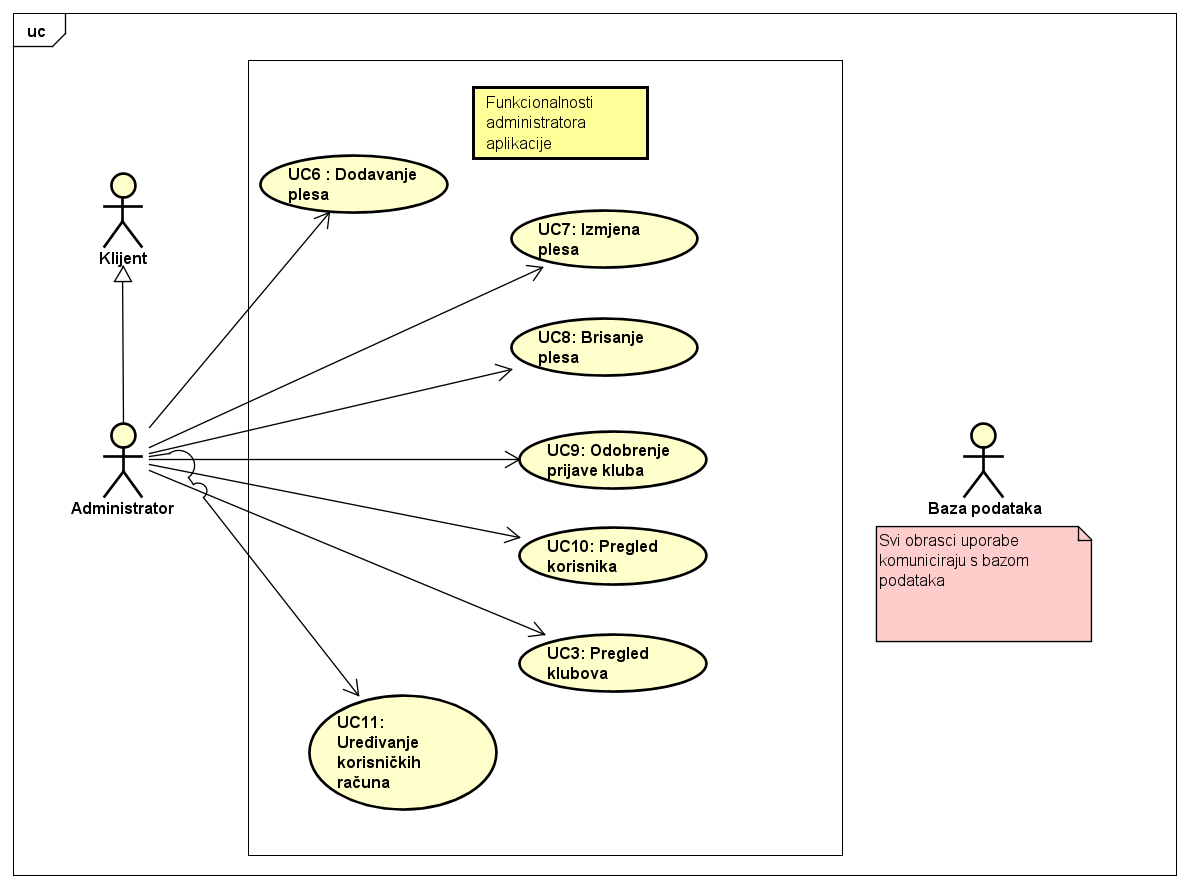
\includegraphics[scale=0.4]{slike/UC_admin.PNG} %veličina u odnosu na širinu linije
			\caption{Dijagram obrasca uporabe, funkcionalnost administratora.}
			\label{fig:UC_admin} %label mora biti drugaciji za svaku sliku
		\end{figure}
		
		
				
			\subsection{Sekvencijski dijagrami}
				
				\textbf{\textit{dio 1. revizije}}\\
				
				\textit{Nacrtati sekvencijske dijagrame koji modeliraju najvažnije dijelove sustava (max. 4 dijagrama). Ukoliko postoji nedoumica oko odabira, razjasniti s asistentom. Uz svaki dijagram napisati detaljni opis dijagrama.}
				\eject
	
		\section{Ostali zahtjevi}
		
			\textbf{\textit{dio 1. revizije}}\\
		 
			 \textit{Nefunkcionalni zahtjevi i zahtjevi domene primjene dopunjuju funkcionalne zahtjeve. Oni opisuju \textbf{kako se sustav treba ponašati} i koja \textbf{ograničenja} treba poštivati (performanse, korisničko iskustvo, pouzdanost, standardi kvalitete, sigurnost...). Primjeri takvih zahtjeva u Vašem projektu mogu biti: podržani jezici korisničkog sučelja, vrijeme odziva, najveći mogući podržani broj korisnika, podržane web/mobilne platforme, razina zaštite (protokoli komunikacije, kriptiranje...)... Svaki takav zahtjev potrebno je navesti u jednoj ili dvije rečenice.}
			 
			 
			 
	